%%%%%%%%%%%%%%%%%%%%%%%%%%%%%%%%%%%%%%%%%
% Daily Laboratory Book
% LaTeX Template 
%
% This template has been downloaded from:
% http://www.latextemplates.com
%
% Original author:
% Frank Kuster (http://www.ctan.org/tex-archive/macros/latex/contrib/labbook/)
%
% Important note:
% This template requires the labbook.cls file to be in the same directory as the
% .tex file. The labbook.cls file provides the necessary structure to create the
% lab book.
%  %%mikeg: Since labbook is installed shouldn't need to do this
% The \lipsum[#] commands throughout this template generate dummy text
% to fill the template out. These commands should all be removed when 
% writing lab book content.
%
% HOW TO USE THIS TEMPLATE 
% Each day in the lab consists of three main things:
%
% 1. LABDAY: The first thing to put is the \labday{} command with a date in 
% curly brackets, this will make a new page and put the date in big letters 
% at the top.
%
% 2. EXPERIMENT: Next you need to specify what experiment(s) you are 
% working on with an \experiment{} command with the experiment shorthand 
% in the curly brackets. The experiment shorthand is defined in the 
% 'DEFINITION OF EXPERIMENTS' section below, this means you can 
% say \experiment{pcr} and the actual text written to the PDF will be what 
% you set the 'pcr' experiment to be. If the experiment is a one off, you can 
% just write it in the bracket without creating a shorthand. Note: if you don't 
% want to have an experiment, just leave this out and it won't be printed.
%
% 3. CONTENT: Following the experiment is the content, i.e. what progress 
% you made on the experiment that day.
%
%%%%%%%%%%%%%%%%%%%%%%%%%%%%%%%%%%%%%%%%%
\documentclass[letterpaper,index=totoc,hyperref,openany]{labbook} % 'openany' here removes the gap page between days, erase it to restore this gap; 'oneside' can also be added to remove the shift that odd pages have to the right for easier reading

%----------------------------------------------------------------------------------------
%	PACKAGES AND OTHER DOCUMENT CONFIGURATIONS
%----------------------------------------------------------------------------------------

\usepackage[ 
%  backref=page, %incompatible with biblatex
  pdfpagelabels=true,
  plainpages=false,
  colorlinks=true,
  bookmarks=true,
  pdfview=FitB]{hyperref} % Required for the hyperlinks within the PDF
  
\usepackage{booktabs} % Required for the top and bottom rules in the table
\usepackage{float} % Required for specifying the exact location of a figure or table
\usepackage{graphicx} % Required for including images

%%Customizations by mikeg
\usepackage{marginnote}%provides ability to put notes in the margin using \marginnote{} coommand
\usepackage{ifthen}
\usepackage{amsmath,amssymb}
\usepackage{xspace}
\usepackage{listings} %provides lstlisting environment for typesetting code
\usepackage[natbib=true,backref=page]{biblatex} %alternative to natbib

\bibliography{/home/mikeg/BiBTeX/bibliography.full}

\usepackage{etoolbox}
\makeatletter
%suppress pagebreaks between days
\patchcmd{\addchap}{\if@openright\cleardoublepage\else\clearpage\fi}{\par}{}{}
%\patchcmd{\scr@startchapter}{\if@openright\cleardoublepage\else\clearpage\fi}{}{}{}
%remove numbering of experiments
%\renewcommand*\theexperiment{}
%\renewcommand*\thesubexperiment{}
\makeatother 

\newcommand{\HRule}{\rule{\linewidth}{0.5mm}} % Command to make the lines in the title page
\setlength\parindent{0pt} % Removes all indentation from paragraphs


%----------------------------------------------------------------------------------------
%	TITLE PAGE
%----------------------------------------------------------------------------------------
\begin{document}
\frontmatter % Use Roman numerals for page numbers
\title{Undergraduate Research Assistant Notes}
\begin{center}
\HRule \\[0.4cm]
{\Huge \bfseries Research Journal \\[0.4cm] % Degree
\HRule \\[1.5cm]}
\end{center}

\author{\LARGE Walker Bussey-Spencer \\ \Large wbusseys@vols.utk.edu \\[2cm]} % Your name and email address
\date{Beginning 22 July 2016} % Beginning date



%\newexperiment{<abbrev>}[<short form>]{<long form>}
%Here, <abbrev> is the abbreviation that can be given later to make LATEX
%use the <long form> and <short form>. The short form is for index, table of
%contents and running title, and giving it is optional. When using the abbre-
%viation, specify it without prepending a backslash, i.e. \experiment{abbrev}.
%Abbreviations may contain any char except the backslash, the tilde ( ̃), comma

\newexperiment{NSE}{NSE SEMPPR}
\newexperiment{ROC}{ROC SEMPPR}
\newexperiment{RPF-ROC}[RPF-ROC]{Ribosome Profile Footprints: Pausing Model}
\newexperiment{RPF-NSE}[RPF-NSE \& ROC]{Ribosome Profile Footprints: NSE \& Pausing Model}
\newexperiment{FONSE}{FONSE SEMPPR}
\newexperiment{DIMCMC}[DIMCMC]{Doubly Intractable MCMC}
\newexperiment{Knight}{Student Learning, Jennifer Knight}
\newexperiment{SELAC}{Main SELAC model}
\newexperiment{Lab}{Lab Meeting}
\newexperiment{LSAs}{LSAs}
\newexperiment{Cedric}{Cedric Landerer}
\newexperiment{Mehmet}{Mehmet Aydeniz}
\newexperiment{SMBE Satellite Meeting on Protein Evolution in Denver}{SMBEDen}
%\newexperiment{shorthand}{Description of the experiment}


%COMMANDS
%%% Sort using M-x 'sort-lines'
\newcommand{\GTR}{GTR+$\Gamma$\xspace}
\newcommand{\LogN}{\ensuremath{\text{LogN}}\xspace}
\newcommand{\Lik}{\ensuremath{\text{\textbf{Lik}}}\xspace}
\newcommand{\LLik}{\ensuremath{\mathcal{L}}\xspace}
\newcommand{\Ne}{\ensuremath{{N_e}}\xspace}
\newcommand{\Piihat}{\ensuremath{\hat{\pi}_i}\xspace}
\newcommand{\Pii}{\ensuremath{\pi_{i}}\xspace}
\newcommand{\Pijhat}{\ensuremath{\hat{\pi}_j}\xspace}
\newcommand{\Pij}{\ensuremath{\pi_{j}}\xspace}
\newcommand{\Pivechat}{\ensuremath{\hat{\Pivec}}\xspace}
\newcommand{\Pivec}{\ensuremath{\Vec{\pi}}\xspace}
%\newcommand{\Pr}{\ensuremath{\text{Pr}}\xspace}
\newcommand{\Qmatrixa}{\ensuremath{\Qmatrix_a}\xspace}
\newcommand{\Qmatrix}{\mathbf{Q}\xspace}
\newcommand{\ROC}{\ensuremath{\text{ROC}}\xspace}
\newcommand{\Var}{\operatorname{Var}}
\newcommand{\var}{\Var}
\newcommand{\Wi}{\ensuremath{{W_i}}\xspace}
\newcommand{\Wj}{\ensuremath{{W_j}}\xspace}
\newcommand{\acivec}{\ensuremath{a\left(\cveci\right)}\xspace}
\newcommand{\acvecg}{\ensuremath{a\left(\vec{c}_{i,g}\right)}\xspace}
\newcommand{\acvecj}{\ensuremath{a\left(\cvecj\right)}\xspace}
\newcommand{\acvec}{\ensuremath{a\left(\Vec{c}\right)}\xspace}
\newcommand{\aip}{\ensuremath{a_{i,p}}\xspace}
\newcommand{\aivecg}{\ensuremath{{\avec}_{i,g}}\xspace}
\newcommand{\aivec}{\aveci}
\newcommand{\ajp}{\ensuremath{a_{j,p}}\xspace}
\newcommand{\ajvecg}{\ensuremath{{\ajvec}_{,g}}\xspace}
\newcommand{\ajvec}{\ensuremath{\Vec{a}_{j}}\xspace}
\newcommand{\aj}{\ensuremath{a__j}\xspace}
\newcommand{\alphac}{\ensuremath{\alpha_c}\xspace}
\newcommand{\alphap}{\ensuremath{\alpha_p}\xspace}
\newcommand{\alphavec}{\ensuremath{\Vec{\alpha}}\xspace}
\newcommand{\alphav}{\ensuremath{\alpha_v}\xspace}
\newcommand{\aobsvecg}{\ensuremath{{\avec}_{\text{obs},g}}\xspace}
\newcommand{\aobsvec}{\ensuremath{\Vec{a}_{\text{obs}}}\xspace}
\newcommand{\aobs}{\ensuremath{a_{\text{obs}}}\xspace}
\newcommand{\aoptip}{\ensuremath{\aopt_{i,p}}\xspace}
\newcommand{\aoptpg}{\ensuremath{\aopt_{p,g}}\xspace}
\newcommand{\aoptp}{\ensuremath{\aopt_p}\xspace}
\newcommand{\aoptvecg}{\ensuremath{{{\aoptvec}_g}}\xspace}
\newcommand{\aoptvec}{\ensuremath{\Vec{a}^*}\xspace}
\newcommand{\aopt}{\ensuremath{{a^*}}\xspace}
\newcommand{\aveci}{\ensuremath{\Vec{a}_i}\xspace}
\newcommand{\avecj}{\ensuremath{\Vec{a}_j}\xspace}
\newcommand{\avec}{\ensuremath{\Vec{a}}\xspace}
\newcommand{\avecopt}{\aoptvec}
\newcommand{\celegans}{\emph{C.~elegans}\xspace}
\newcommand{\cveci}{\ensuremath{\cvec_i}\xspace}
\newcommand{\cvecj}{\ensuremath{\cvec_j}\xspace}
\newcommand{\cvec}{\ensuremath{\Vec{c}}\xspace}
\newcommand{\deltaT}{\ensuremath{\delta t}\xspace}
\newcommand{\ecoli}{\emph{E.~coli}\xspace}
\newcommand{\Lklu}{\emph{L.~kluyveri}\xspace}
\newcommand{\bsubtilis}{\emph{B.~subtilis}\xspace}
\newcommand{\fij}{\ensuremath{f_{i,j}}\xspace}
\newcommand{\gen}{\ensuremath{\text{gen}}\xspace}
\newcommand{\jmax}{\ensuremath{{j_{\max}}}\xspace}
\newcommand{\kmax}{\ensuremath{{k_{\max}}}\xspace}
\newcommand{\muij}{\ensuremath{\mu_{i,j}}\xspace}
\newcommand{\phiROC}{\ensuremath{\phi_\ROC}\xspace}
\newcommand{\phig}{\ensuremath{\phi_{g}}\xspace}
\newcommand{\pij}{\ensuremath{p_{i,j}}\xspace}
\newcommand{\qij}{\ensuremath{q_{i,j}}\xspace}
\newcommand{\qji}{\ensuremath{q_{i,j}}\xspace}
\newcommand{\rib}{\ensuremath{\text{rib}}\xspace}
\newcommand{\cell}{\ensuremath{\text{cell}}\xspace}
\newcommand{\sphi}{\ensuremath{s_\phi}\xspace}
\newcommand{\scer}{\emph{S.~cerevisiae}\xspace}
\newcommand{\setG}{\ensuremath{\mathbb{G}}\xspace}
\newcommand{\setP}{\ensuremath{\mathbb{P}}\xspace}
\newcommand{\setC}{\ensuremath{\mathbb{C}}\xspace}
\newcommand{\setF}{\ensuremath{\mathbb{F}}\xspace}
\renewcommand{\ng}{\ensuremath{{n_g}}\xspace}
\newcommand{\researcher}{\subsubsection}
%---------------------------------------------------------------------------------------

\graphicspath{{./Figures//}} % double slash indicates search recursively within folder
%%Figures will be organized in subfolders by year/month
\DeclareGraphicsExtensions{.pdf, .png, .jpg} %prevent the need for using file extensions

\begin{document}

\frontmatter

\maketitle

\tableofcontents

\mainmatter % Use Arabic numerals for page numbers

%----------------------------------------------------------------------------------------
%	LAB BOOK CONTENTS
%----------------------------------------------------------------------------------------

% Blank template to use for new days:

%\labday{Day, Date Month \Year}

%\experiment{}

%Text

%-----------------------------------------

%\experiment{}

%\begin{figure}[H] % Example of including images
%\begin{center}
%\includegraphics[width=0.5\linewidth]{example_figure}
%\end{center}
%\caption{Example figure.}
%\label{fig:example_figure}
%\end{figure}

%Text

%----------------------------------------------------------------------------------------
%each sentence gets its own line!


\labday{22 July 2016}
\experiment{C. Elegans Life Stages}
\researcher{Walker Bussey-Spencer}
\begin{itemize}
  \item Looking at data with original model— accounting for noise and include an intercept
  \item Created 2 non-overlapping sets out of the life stages
    \begin{itemize}
	\item First set includes more data points and is called “lower hierarchy” 
	\item Second set includes fewer, more encompassing data points and is called “higher hierarchy”
    \end{itemize}
  \item Running the MCMC with each of these different selected data sets.
  \end{itemize}

\begin{figure}
\centering
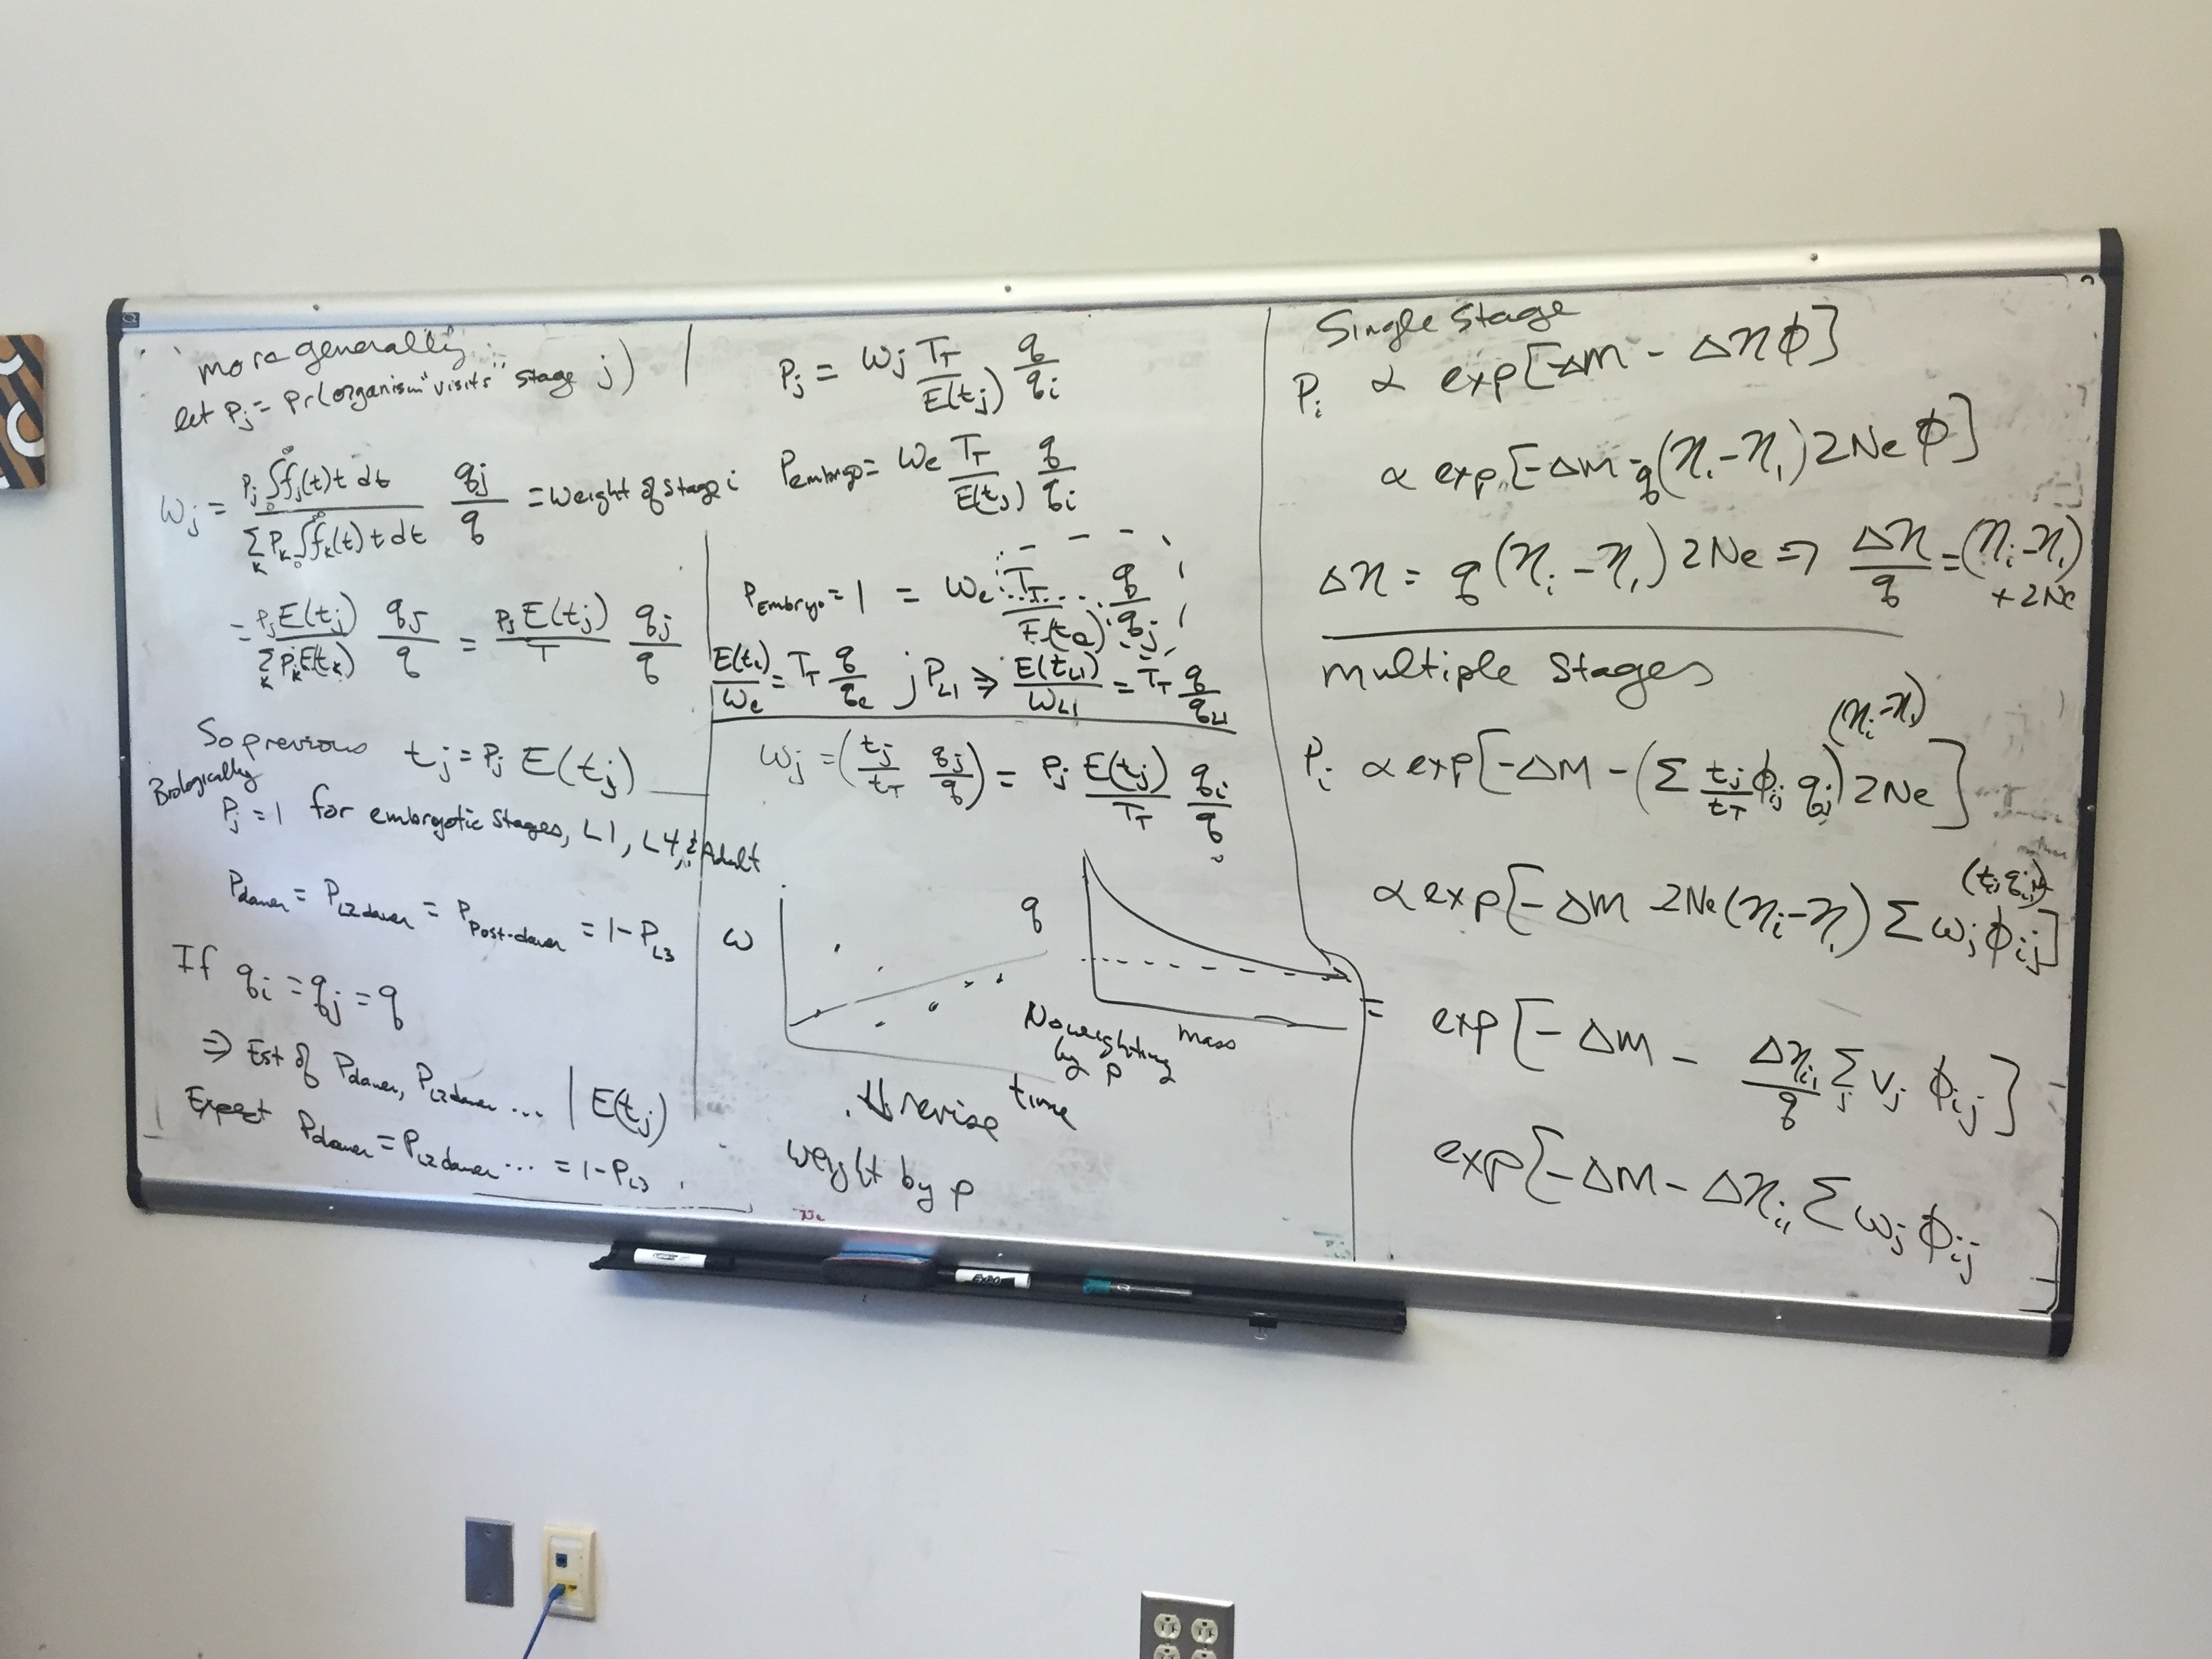
\includegraphics[scale=.65]{../Figures/2016/July_22/OmegaDerivation.jpg}
\caption{Derivation of Expression Coefficient as Multivariable Function}
\label{fig:JUL24_MATH}
\end{figure}

\begin{itemize}
\item Meeting with Dr. Gilchrist:
\item On the far right of fig:JUL24_MATH, we derived the weighting coefficient/expression coefficient omega as a function of time and ATP cost importance.
\item Then, to handle the fact that we do not necessarily know the length of time stages or the definite occurrence of each time stage, we defined omega in terms of the probability of observing a given time stage for a certain amount of time divided by the total proabability.
\item There was also a factor of the cost importance in the particular stage compared to probably the overall cost importance.
\item We established that the probability of observing a certain life stage was = 1 for the life stages which are inevitable for the C. Elegans, specifically: the embryonic stages, L1, L4, and Adult stage.
\item The probability of observing dauer, l2 dauer, and post dauer were all equal, and also were equal to 1 - probability of entering L2/L3.
\item The last formula we arrived at was that the probability of a life stage is equal to the the product of the omega, the total time, and the average ATP cost divided by the product of the expected value of the time in the life stage and the life stage specific q value.
\item Since we know the expected time value and the omega value, we can obtain ratio values for the different q values, as the total time and average q can cancel out.
\item We also can look at the assumption that the embryonic stages all have the same relative q values since there is a limited amount of energy in the egg that does not change in a ratio between life stages.
\item The first step now is to write two codes that include all the dauer stages and differ only in the accounting for the two aforementioned non-overlapping sets.
\item To Do:
\begin{itemize}
\item Address how the measurements in a stage that consists of substages is generated.
\item Find out where Cedric got the data.
\item Look at how the mass of the worm changes with each life stage to gain insight into the q values.
\item Make sure sum of weighting constraints = 1.
\item Write the code for each set.
\end {itemize}
\end{itemize}

\labday{25 July 2016}
\experiment{C. Elegans Life Stages}
\begin{itemize}
\item Morning Meeting:
\begin{itemize}
\item Look up what unit testing is.
\item Look up mortality Leslie matrix.
\item Look up Hawk and Dove game.
\end{itemize}
\item Trying to gain comfort and ability with this latex program.
\item Asked Cedric where he got the life stages data and he gave me the link to the website:
\item 
\end{itemize}
\end{document}






%git add .


